\newcommand\domain[3]{Let $\Omega\subseteq\reals^{#2}$, and ${#1}:\Omega \to \reals^{#3}$}
\chapter{Functions of Several Variables}
\setcounter{exercisecounter}{0}
\setcounter{thmcounter}{1}

We now relax the conditions that functions have to be linear. Moreover, we can restrict the domain of the function to be some subset $\Omega \subseteq \reals^n$, as some functions are not everywhere defined on $\reals^m$.

\example{
    Find the largest domain $\Omega\subseteq\reals^3$ such that the function \[
        f(x,y,z)=\frac{1}{x^2+y^2+z^2-9}   
    \]
    is defined.
}
The right hand side is well defined for any $x^2+y^2+z^2-9\neq 0$. That is, you can calculate the right hand side as long as you are not dividing by zero. This means we can take the largest domain to be $\Omega = \reals^3 - \{(x,y,z)|x^2+y^2+z^3=9\}$. What is this mysterious region described by $x^2+y^2+z^2=9$? Recall that $\sqrt{x^2+y^2+z^2}$ is distance of $(x,y,z)$ from the origin, so this traces out a sphere of radius $3$.

\section{Graphing in $\reals^n$}

Graphing has always been a useful tool for to gain intuition about the `shape' of functions. Here we formalize the definition of the graph of a function.

\definition{Graph}{
    \domain{f}{n}{}. We denote the \textbf{Graph} of $f$ to be $\Gamma_f$, and is the subset of $\reals^{n+1}$ \[
    \Gamma_f\defeq\{(\vec{x},f(\vec{x})) \ |\ \vec{x}\in\Omega\}.
    \]
}
Intuitively, this means we take $\Omega$ and lift that set in the $(n+1)$-st dimension according to the value of $f(\vec{x})$ evaluated at each point.
\example{
    Let $f(x,y)=(49+3x-2y)/6$, then the graph of $f$ is a plane in 3D space, which we have sketched in \hyperref[ex:1.26]{one example} in the first chapter.
}

This is not too hard to understand for one or two variables, but gets out of hand quickly as $n$ increases. I sometimes struggle to visualize even in the third dimension. One way to get around this is to look at the cross sections of a graph. 
\definition{Level set}{
    \domain{f}{n}{}. Let $c\in \reals$. The \textbf{level set} of $f$ at $c$ is denoted $L_c$, and is the set \[
    L_c\defeq \{\vec{x}\in\Omega \ | \ f(\vec{x})=c\}.
    \]
}
Why is this a natural definition? Consider the the intersection between $\Gamma_f$ and the hyperplane described by the set of $(\vec{x},c)$ for all $\vec{x}\in \reals^n$. This plane will intersect all the points in $L_c$, except they are lifted in the $(n+1)$-st dimension by $c$ units. That is, if you understand how all the $L_c$'s behave for all values of $c$, you understand how the graph of $L_c$ behaves.

\example{
    What are the level sets of the function $f(x,y)=\sqrt{x^2+y^2}$? 
}
The function here is not complicated at all: This is the distance $(x,y)$ from the origin, meaning the graph of $f$ is a cone. If we take cross section slices of positive heights, we will get circles. For negative heights, we get an empty set. For $c=0$, $L_c$ only contains the origin.

We can compress these level sets back to 2 dimensions.
\begin{figure}[h]
    \begin{subfigure}[l]{0.46\textwidth}
    \centering
    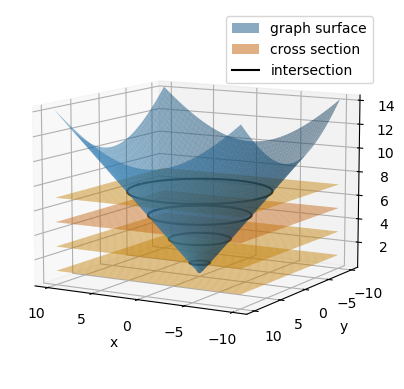
\includegraphics[width=\textwidth]{Rn_function/cone.png}
    \caption{Cross sections of the cone}
    \end{subfigure}
    \begin{subfigure}[r]{0.5\textwidth} 
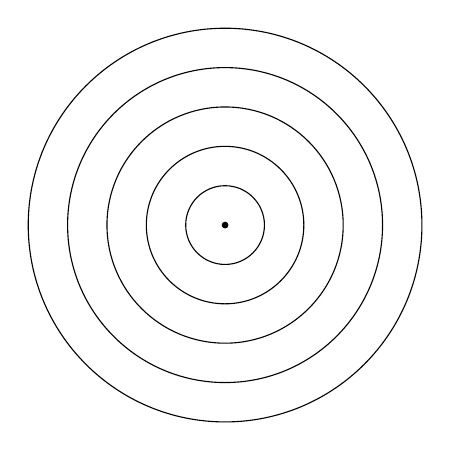
\begin{tikzpicture}
    \filldraw(0,0) circle(1pt);
    \draw (0,0)circle (0.5);
    \draw (0,0)circle (1);
    \draw (0,0)circle (1.5);
    \draw (0,0)circle (2);
    \draw (0,0) circle(2.5);
\end{tikzpicture}
\caption{The level sets $c=0$ to $c=5$, evenly spaced}.
    \end{subfigure}
\end{figure}

Let us see how our flatlander friend Frankie (apparently that is what the inhabitants of $\reals^2$ call themselves) can visualize this cone from the 2D level sets. Frankie holds a meter that constantly evaluates $f(x,y)$ at any point. He realizes that if he circles the origin at a radius of $r$, the meter will stay constant at a value of $r$. If he walks directly away from the origin, the meter will increase in value. Moreover, because the level sets $L_1,L_2,L_3,L_4,...$ are evenly spaced, Frankie only needs to walk a the same distance away from the origin to raise the meter value the same amount. Translated back to 3D, Frankie is actually `hiking' up the cone as he walks away from the origin. The slope (evaluated from the radial cross section) is $1$, so Frankie walks $k$ units away from the origin to raise his elevation by $k$, no matter where he is.

\example{
    What are the level sets of the function $f(x,y,z)={x^2+y^2+z^2}$? 
}
Now we play the role of Frankie. 

First we try to see what the level sets $f(x,y,z)=c$ look like. This is a sphere of radius $\sqrt(c)$. The level sets are also spheres, but this time they are spaced a little bit different. To go from the level set $L_c$ to $L_{c+1}$, we go from the sphere of radius $\sqrt{c}$ to $\sqrt{c+1}$, and the shortest distance is  \[
    \sqrt{c+1}-\sqrt{c} =  \frac{(\sqrt{c+1}-\sqrt{c})(\sqrt{c+1}+\sqrt{c})}{(\sqrt{c+1}+\sqrt{c})} = \frac{1}{\sqrt{c+1}+\sqrt{c}}
\]
which gets smaller as $c$ increases! This means we need to walk a shorter distance to increase our meter. Equivalently, the `slope' in this direction increases as we get further away.

\example{Sketch the function $f(x,y)=xy$, either in 3D or through its 2D level sets.}

Let us begin by considering the level sets $xy=c$. This describes the graph $y=c/x$, except for the case $c=0$, then the level set is the x and y axes.
\begin{figure}[h]
    \centering
    \begin{subfigure}{0.48\textwidth}
        \centering
        \begin{tikzpicture}
            \draw[->] (-4, 0) -- (4, 0) ;%node[right] {$x$};
            \draw[->] (0, -4) -- (0, 4) node[above] {$y$};
            %\foreach \i in {1,..,3}{
            \draw[scale=1, domain=-4:-0.25, smooth, variable=\x, blue] plot ({\x}, {1/\x});
            \draw[scale=1, domain=-4:-0.5, smooth, variable=\x, blue] plot ({\x}, {2/\x});
            \draw[scale=1, domain=-4:-0.75, smooth, variable=\x, blue] plot ({\x}, {3/\x});
            \draw[scale=1, domain=0.25:4, smooth, variable=\x, blue] plot ({\x}, {1/\x});
            \draw[scale=1, domain=0.5:4, smooth, variable=\x, blue] plot ({\x}, {2/\x});
            \draw[scale=1, domain=0.75:4, smooth, variable=\x, blue] plot ({\x}, {3/\x});
            %}
          \end{tikzpicture}
          \caption{Positive $c$}
    \end{subfigure}
    \begin{subfigure}{0.48\textwidth}
        \centering
        \begin{tikzpicture}
            \draw[->] (-4, 0) -- (3.9, 0) node[below right ] {$x$};
            \draw[->] (0, -4) -- (0, 4) node[above] {$y$};
            %\foreach \i in {1,..,3}{
            \draw[scale=1, domain=-4:-0.25, smooth, variable=\x, red] plot ({\x}, {-1/\x});
            \draw[scale=1, domain=-4:-0.5, smooth, variable=\x, red] plot ({\x}, {-2/\x});
            \draw[scale=1, domain=-4:-0.75, smooth, variable=\x, red] plot ({\x}, {-3/\x});
            \draw[scale=1, domain=0.25:4, smooth, variable=\x, red] plot ({\x}, {-1/\x});
            \draw[scale=1, domain=0.5:4, smooth, variable=\x, red] plot ({\x}, {-2/\x});
            \draw[scale=1, domain=0.75:4, smooth, variable=\x, red] plot ({\x}, {-3/\x});
            %}
          \end{tikzpicture}
          \caption{Negative $c$}
    \end{subfigure}
\end{figure}


\begin{wrapfigure}{l}{0.4\textwidth}
    \centering
    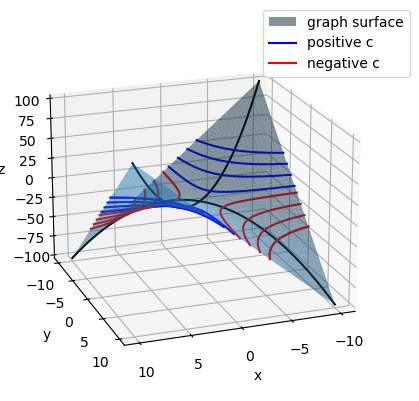
\includegraphics[width=0.4\textwidth]{Rn_function/saddle.png}
    %\caption{The surface $f(x,y)=xy$}
\end{wrapfigure} There are many ways to visualize the actual surface from here: My goto way is to vary $c$ and see how the level set changes. In this case, starting from positive $c$ and decreasing, the curves get closer and closer to the $x$ and $y$ axis, and they `flip' across the axis as the sign of $c$ changes from positive to negative.

The graph looks something like a saddle, or a pringle chip. Saddle points are somewhere between a local maximum and a local minimum. The saddle point of this function is at the origin: going the direction of $x=y$, you will get $f(x,y)=x^2$ that curves upwards; going in the direction of $x=-y$, you get $f(x,y)=-x^2$ which curves downwards. This point is \textit{in some sense} a local minimum and a local maximum depending on which way you look at it.


\example{Let $a,b,c>0$, and $k,m,l\in\reals$. What does the surface described by \[
    \frac{x^2-2kx}{a^2}+\frac{y^2-2my}{b^2}+\frac{z^2-2lz}{c^2}=1
\]
look like?
}
Let us approach a simplier version of the problem first: what is the surface described by \[
    \frac{x^2}{a^2}+\frac{y^2}{b^2}+\frac{z^2}{c^2}=1?
\]
We know what happens when $a=b=c=1$. Namely, we get the unit sphere. Now if we stretch the x axis by a factor of $a$, we will change from a surface \[
    x^2+y^2+z^2=1 \to \frac{x^2}{a^2}+y^2+z^2=1!
\]
Because the x,y,z axes are orthgonal, we can also stretch the y and z axes by a factor $b$ and $c$ respectively to give the surface. This will give us an ellipsoid, which is just a stretched (or compressed) sphere. To deal with the original equation, we can complete the square to get \begin{align*}
    \frac{x^2-kx}{a^2}+\frac{y^2-my}{b^2}+\frac{z^2-lz}{c^2}&=  \frac{(x-k)^2-k^2}{a^2}+\frac{(y-m)^2-m^2}{b^2}+\frac{(z-l)^2-l^2}{c^2}\\
    &=\frac{(x-k)^2}{a^2}+\frac{(y-m)^2}{b^2}+\frac{(z-l)^2}{c^2} -\frac{k^2}{a^2}-\frac{m^2}{b^2}-\frac{l^2}{c^2}, \\
\end{align*}
Which means we have an ellipsoid but now translated $(k,m,l)$ units!
In the later exercises, you will classify the surfaces described by \[
    x^2+y^2-z^2=1, \ x^2-y^2-z^2=1,
\]
which are called one and two sheeted hyperboloids respectively. 

In later chapters we will see a way to change our coordinate system, through some rotation, scaling and translation, to make any surface in the form \[
    ax^2+by^2+cz^2+dxy+eyz+fzx+gx+hy+iz=j
\] look similar to that of a ellipsoid, one sheet hyperboloid, or a two sheet hyperboloid.
